In step 3 of GDDA, we have to decide the value for the imitation parameter. According to \eqref{eq:lambda_constraint}, to achieve the best performance of the target model, the imitation parameter should be set to minimize the training error. In this section, we illustrate our method GDDA-SVM that uses SVM as the base learner and can effectively estimate the imitation parameter.
\subsection{Distillation with multiple sources}
As we discussed Section \ref{sec:key}, we should find a method that can estimate the optimal imitation parameter effectively for real applications. 
To solve this problem, we propose a novel method that can determine the imitation parameter $\lambda$ autonomously, called GDDA-SVM. In our GDDA-SVM, instead of using cross-entropy loss, we use Mean Squared Error (MSE) as our loss function for the following two reasons: (1) Some recently work \cite{ba2014deep,luo2016face,romero2014fitnets,urban2016deep} show that MSE is also an efficient measurement for the targets model to mimic the behavior of the source model. (2) MSE can provide a closed form cross-validation error estimation and help us to choose the proper imitation parameter effectively. 

\begin{figure}
\centering
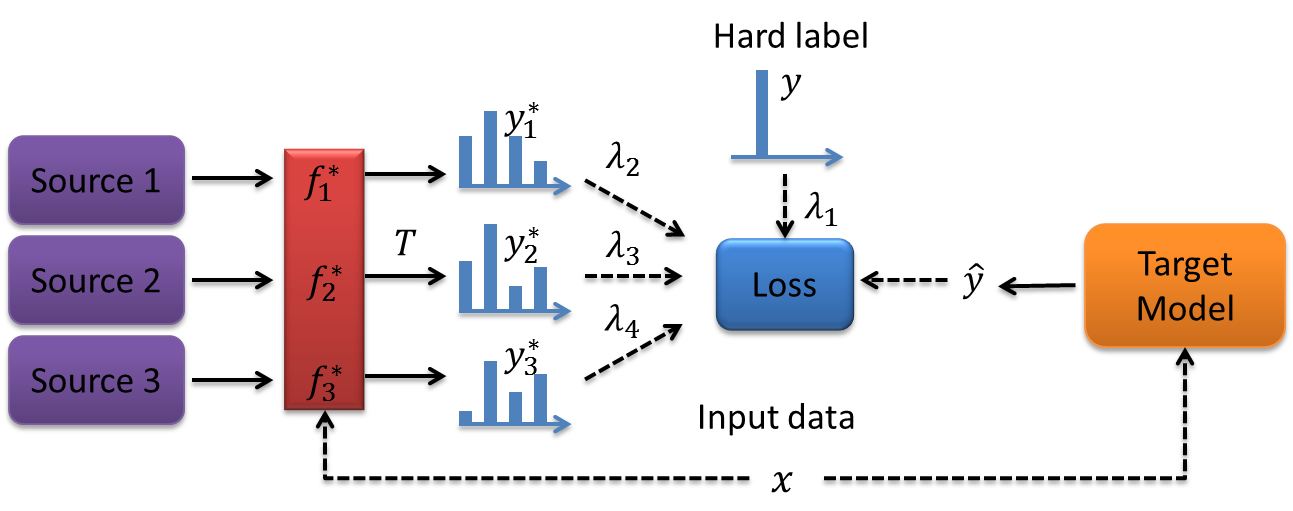
\includegraphics[scale=.4]{figure/multi-GDDA.png}
\caption{Illustration of GDDA training process.}
\end{figure}

Suppose we have $L$ examples $\{x_i,y_i\}_{i=1}^L$ from and $N$ classes in the target domain where $X\in R^{L\times d}, Y\in R^{L\times N}$. Meanwhile, there are $M-1$ the source (teacher) models providing the soft labels $\{Y^*_i\}_{i=1}^{M-1}$ for each of the $L$ examples.
For simplicity, we combining the hard label $Y$ and soft label $Y^*$ and use new label matrix: $S = R^{M\times L \times N}$ to denote them. To solve this $N$-class classification problem, we adopt the One-vs-All strategy to build $N$ binary SVMs.
To obtain the $n$th binary SVM, we have to solve the following optimization problem: 
\begin{equation}\label{eq:multi-distill}
\begin{aligned}
\min \qquad & \frac{1}{2}{\left|| w_n \right||^2} + C\sum_{i,j} \lambda_i{e_{ijn}^2} \\
s.t.\qquad& e_{ijn} = s_{ijn} - w_nx_j\\
& \sum_i\lambda_i=1\\
& \lambda_i \in [0,1]; i\in M;  j\in L\\
\end{aligned}  
\end{equation}
To solve this optimization problem, we use KKT theorem \cite{cristianini2000introduction} and add the dual sets of variables to the Lagrangian of the optimization problem:
\begin{equation}
\begin{aligned}
\mathcal{L}=&\frac{1}{2}{\left| w_n \right|^2} + C\sum_{i,j} \lambda_i{e_{ijn}^2}+\sum_{i,j}\alpha^{(n)}_{ij}\left(s_{ij} - wx_j-e_{ij}\right)\\&+\beta^{(n)}\left(\sum_i\lambda_i-1\right)
\end{aligned}
\end{equation}
To find the saddle point, 
\begin{equation}
\begin{aligned}
\frac{{\partial L}}{{\partial w_n}}& = w_n - \sum_{j}\alpha^{(n)}_{ij} {x_j}=0 \rightarrow w_n = \sum_{j}\alpha^{(n)}_{ij} {x_j}\\
\frac{{\partial L}}{{\partial {e_{ijn}}}} & = 2C\lambda_i {e_{ijn}} - {\alpha^{(n)} _{ij}}=0 \rightarrow \alpha^{(n)}_{ij} = 2C\lambda_i {e_{ijn}}\\
\end{aligned}
\end{equation}
For each example $x_j$ and its constraint of label $s_{ijn}$, we have $e_{ijn}  + w_nx_j= s_{ijn}$. Replacing $w_n$ and $e_{ijn}$,  we have:  
\begin{equation}
\begin{aligned}
%x_j\sum_{k}\alpha^{(n)}_{ik}x_k+\frac{\alpha^{(n)}_{ij}}{2C\lambda_i}&=s_{ijn}\\
\lambda_ix_j\sum_{k}\alpha^{(n)}_{ik}x_k+\frac{\alpha^{(n)}_{ij}}{2C}&=\lambda_is_{ijn}
%x_j\sum_{k}\alpha^{(n)}_{ik}x_k+\sum_j\frac{\alpha^{(n)}_{ij}}{2C}&=\sum_j\lambda_js_{ijn}
\end{aligned}
\end{equation}
Summing over each constraint of example $x_j$, we have:
\begin{equation}
\underbrace{\sum_i\lambda_i}_{=1} x_j\sum_{k}\alpha^{(n)}_{ik}x_k+\sum_i\frac{\alpha^{(n)}_{ij}}{2C}=\sum_i\lambda_is_{ijn}
\end{equation}
%Here we use $K$ to denote the kernel matrix $K=\{x_ix_j|i,j\in 1\dots L\}$.
Let %$M=[K+\frac{\mathbf{I}}{2C}]$ and 
$\eta_{jn}=\sum_i\alpha^{(n)}_{ij}$, we have:
\begin{equation}
\begin{aligned}
\sum_j\eta_{jn}x_jx_i+\frac{\eta_{in}}{2C}&=\sum_i\lambda_is_{ijn}\\
%M\eta_n&=S_n\begin{bmatrix}
%\lambda_1\\\vdots\\\lambda_m
%\end{bmatrix}
\end{aligned}
\end{equation}

This implies that solving the optimization problem \eqref{eq:multi-distill} is equivalent to solve a standard LS-SVM whose the target is encoded as $\sum_i\lambda_is_{ijn}$, i.e. the weighted label matrix $S$.

Here we use $\Omega$ to denote the matrix $\Omega=[K+\frac{\mathbf{I}}{2C}]$ where $K$ is the kernel matrix $K=\{x_ix_j|i,j\in 1\dots L\}$. To simplify our notation, let ${\eta}'_{n}=M^{-1}S_n$ where $S_n$ is the matrix $S_n=\{s_{ijn}|i\in M;j\in L\}$ and $\Omega^{-1}$ is the inverse of matrix $\Omega$. 

Let $\eta_{jn}=\sum_i\lambda_i{\eta}'_{ijn}$.
The Leave-one-out estimation of the example $x_j$ for the $n$th binary SVM can be written as \cite{cawley2006leave}:
\[\sum_i\lambda_is_{ijn}-\hat{y}_{jn} =\frac{{\eta}_{jn}}{\Omega_{jj}^{-1}} =\frac{\sum_i\lambda_i{\eta}'_{ijn}}{\Omega_{jj}^{-1}}\]
\begin{equation}\label{eq:yhat}
\hat{y}_{jn} = \sum_i\lambda_i\left(s_{ijn}-\frac{{\eta}'_{ijn}}{\Omega_{jj}^{-1}}\right)
\end{equation}
where $\Omega^{-1}_{jj}$ is the $j$th diagonal element of $\Omega^{-1}$. Now, we have found an efficient way to estimate the output of each binary student model for example $x_j$. In the following part, we will introduce how to find the optimal $\lambda_i$ for each of the source models. 
\subsection{Cross-entropy loss for imitation parameter estimation}
From the previous part, we have already found a effective way to estimate the output of the SVM. The optimal imitation parameters, can be found by solving the following optimization problem:
\begin{equation}\label{eq:loo_loss}
\begin{aligned}
\min \quad& L_c\left(\lambda\right)=\frac{1}{2}\sum_i^M||\lambda_i||^2+\frac{1}{L}\sum_{j,n}\ell\left(y_{in},\hat{y}_{jn}\left(\lambda\right)\right)
\end{aligned}
\end{equation}
Here we use the L2 regularization term to control the complexity of $\lambda$ so that the estimated $\lambda$ can perform well on the testing data. For the loss $\ell(\cdot)$, We choose the cross-entropy (CE) as the loss function.
Compared to MSE, cross-entropy pay less attention to a single incorrect predicted example which reduced the affect of the outliers in the training data. Moreover, cross-entropy works better with unlabeled data. As we mentioned in our "fake label" strategy, we use one-hot strategy to encode the hard labels of the labeled examples while encoding the unlabeled examples with gray code. When we use cross-entropy, it can ignore penalties of the unlabeled example and limit the noise introduced by our "fake label" strategy. Therefore, 
Let:
\begin{equation}\label{eq:mu}
\begin{aligned}
\mu_{ijn}=s_{ijn}-\frac{{\eta}'_{ijn}}{\Omega_{jj}^{-1}} \qquad
P_{jn} = \frac{e^{\hat{y}_{jn}}}{\sum_{h} e^{\hat{y}_{jh}}}
\end{aligned}
\end{equation}
The derivative can be written as:
\begin{equation}\label{eq:p}
\begin{aligned}
\frac{\partial \ell(\lambda)}{\partial \lambda_i}&=\sum_n\mu_{ijn}\left(P_{jn}-{y}_{jn}\right)
\end{aligned}
\end{equation}
\begin{algorithm}[t]
	\caption{GDDA-SVM}\label{alg:svm}
	\begin{algorithmic}
		\Require Input examples $X=\{x_1,...,x_L\}$, number of classes $N$, size of sources $M$, 3D label matrix, $S=[Y_1,Y_2,...,Y_{M}]$ with size $L\times M \times N$, temperature $T$, optimization iteration $iter$
		\Ensure Target model $f_t = Wx$
		\State Compute $\Omega=[K+\frac{\mathbf{I}}{2C}]$
		\State Compute imitation parameter $\lambda$ with Algorithm \ref{alg:lambda}
		\State Compute new label $Y_{new}=\sum_i\lambda_iY_i$
		\State Compute $\eta = \Omega^{-1}Y_{new}$
		\State Compute $w_n = \sum_j \eta_{jn}x_j$
	\end{algorithmic}	
\end{algorithm}
\begin{algorithm}
	\caption{$\lambda$ Optimization}\label{alg:lambda}
\begin{algorithmic}
	\Require Input examples $X$, number of classes $N$, size of sources $M$, 3D label matrix $S$, temperature $T$, optimization iteration $iter$, Kernel matrix $\Omega$
    \Ensure Imitation parameter $\lambda$
    \State Initialize $\lambda = \frac{1}{M}$, 
    
    \State Let $S_n$ be the label matrix of $S$ for class $n$
    \For{Each label $S_n$} 
    \State Compute $\eta'_n=\Omega^{-1}S_n$ 
    \EndFor
    \State Compute $\mu$ using \eqref{eq:mu}
    \For {$it \in iter$ }
	    \State Compute $\hat{y}_{jn}$ and $P_{jn}$ with \eqref{eq:yhat}  and \eqref{eq:p}
	    \State $\Delta_{\lambda} \leftarrow 0$
	    \For {each $x_j$ in $X$}
		    \State $\Delta_{\lambda} = \Delta_{\lambda}+\sum_n\mu_{ijn}\left(P_{jn}-{y}_{jn}\right)$
	    \EndFor
	    \State $\Delta_{\lambda} =\Delta_{\lambda}/L$, $\lambda = \lambda - \frac{1}{itr}(\Delta_{\lambda}+\lambda)$
%	    \State 
    \EndFor
\end{algorithmic}	
\end{algorithm}
In addition, we describe GDDA-SVM in Algorithm \ref{alg:svm}. As the optimization problem \eqref{eq:loo_loss} is strongly convex, it is easy to proof that Algorithm \ref{alg:lambda} can converge to the optimal $\lambda$ with the rate of $O(\log(t)/t)$ where $t$ is the optimization iteration\footnote{The proof is similar to the proof of Lemma 1 in \cite{shalev2011pegasos}.}. 




